So far, we have only considered methods to sample static averages, which concern quantities at thermodynamic equilibrium.
Such techniques yield information about the bulk macroscopic properties of the system, for which there is no discernable macroscopic evolution.
We now turn to the next natural question, which is to consider systems in which there is such an evolution,
 which typically arises from a perturbation of the equilibrium dynamics, either by the introduction of a non-gradient forcing term, 
 or a modification of the fluctuation-dissipation part for which the fluctuation-dissipation relation \eqref{eq:general_fd_relation} is not satisfied.
 We will not consider the latter case, which is relevant for instance to the modelling of heat transport within an atomic system, to concentrate on the first case.
 In general, systems undergoing such a perturbation of the dynamics will reach a new steady state in which there is a net flux in some observable.
 Mathematically, this translate into the existence of a response observable $R$ which has zero average with respect to the canonical measure $\mu$, but which has a non-zero average with respect to the perturbation steady-state.
 A natural question is that of the sensitivity of the system to the perturbation: one way to quantify this is to modulate the strength of the perturbation by a positive real parameter $\eta>0$, and,
  assuming that the average response is asymptotically linear as $\eta\to 0$, to compute the linear coefficient linking $\eta$ and the average response. 
  This quantity is called a \textit{transport coefficient}, and we will dedicate the next two chapters to different methods of computing them using molecular simulation.
  We consider the most natural method, which is to directly apply a forcing term which does not arise from a potential. 
  The mathematical translation of this idea is a Langevin dynamics with an additional non-gradient forcing term. 
  We start by presenting the general framework of non-equilibrium molecular dynamics (NEMD), the numerical methods we implemented, and the examples of shear viscosity and mobility. We illustrate these examples with numerical results.
  We then turn to discussing the Green--Kubo method, which allows for the computation of transport coefficients from equilibrium simulations, before applying it to the same examples as in the previous section.

\section{Non-equilibrium molecular dynamics}
\subsection{General framework}
We consider the following modified Langevin dynamics:
\begin{equation}
    \label{eq:general_nemd_dynamics}
    \left\{\begin{aligned}
        \text dq_t&=M^{-1}p_t\dt,\\
        \text dp_t&= -\nabla V(q_t)\dt -\gamma M^{-1}p_t\dt+\sqrt{\frac{2\gamma}\beta}\text dW_t +\eta F(q_t)\dif t,
    \end{aligned}\right.
\end{equation}
perturbed by the configuration-dependent forcing term $F$, and where the strength of the perturbation is modulated by the parameter $\eta>0$.
Its generator is given by the operator 
\begin{equation}
    \label{eq:nemd_generator}
    \cL_{\gamma,F}=\cL_\gamma +\eta F\cdot \nabla_p = \cL_\gamma +\eta \widetilde{\cL}.
\end{equation}
It is also possible to consider non-equilibrium generalized Langevin equations, which are analogous perturbations of \eqref{eq:general_langevin}.
Given a response of interest $R$, the transport coefficient is given by the following definition:

\begin{equation}
    \label{eq:transport_coefficient}
    \rho_{R,F}=\underset{\eta \to 0}{\lim}\, \frac{\mathbb{E}_\eta[R]}{\eta},
\end{equation}
where $\mathbb{E}_\eta$ denotes the expectation with respect to the steady-state probability distribution. 
If the context makes $R$ clear from the knowledge of $F$, we will drop it from the notation and simply write $\rho_F$ for the transport coefficient.
For this definition to make sense, one has to show that the steady-state with respect to which we take the expectation is well-defined.
Since the steady-state is defined by the fact that it is invariant with respect to the dynamics \eqref{eq:general_nemd_dynamics}, 
this translate into the fact that it is the solution to a stationary Fokker-Planck equation, in the sense of distributions:
\begin{equation}
    \label{eq:nemd_fp_equation}
    (\cL_\gamma +\eta \widetilde{\cL})^\dagger \psi_\eta = 0,
\end{equation}
where $\psi_\eta$ is the steady state measure. Using analytic properties of $\cL_{\gamma,F}$ (such as hypoellipticity), one can hope to infer regularity results of its solutions, such as the existence of a smooth density.
Existence of the steady-state can hopefully be obtained using Lyapunov techniques.
The steady-state measure $\E_\eta$ is a high-dimensional measure on phase space for which a closed form is generally unavailable.
Thus, as usual, one has to resort to ergodic averages under the dynamics \eqref{eq:general_nemd_dynamics} to compute ensemble averages.
This poses another theoretical difficulty, that of showing that the steady-state measure is ergodic, although in principle, uniqueness and ergodicity in the sense of convergence of averages can in principle be recovered following Klieman's method \cite{K87}. 

In fact, for our purposes, $F$ will always be $L$-periodic, and so we can invoke a special case of Proposition 1 in \cite{JPS15} with time-constant forcings, provided $V$ and $F$ are smooth.
\begin{theorem}[Existence of a unique ergodic measure with smooth density]\label{thm:nemd_exst_invariant_measure}
    Let $\eta_*>0$. For all $\eta\in[-\eta_*,\eta_*]$, the Fokker-Planck equation \eqref{eq:nemd_fp_equation} admits a unique solution with a $C^\infty$ density $\psi_\eta$.
    Additionally, the evolution semigroup decays exponentially in a Lyapunov sense: for all $n\geq 1$, there exist $C_n,\,\lambda_n>0$ such that
    \begin{equation}
        \label{eq:lyapunov_exp_decay}
        \left\|\e^{t\cL_{\gamma,F}}\varphi-\E_\eta[\varphi]\right\|_{B^{\infty}(\mathcal E)}\leq C_n\e^{-\lambda_n t}\|\varphi\|_{B^\infty_{\mathcal K_n}},
    \end{equation}
    where we define the Lyapunov weight functions
    \[\mathcal K_n(q,p)=1+|p|^{2n},\]
    and the corresponding $B^{\infty}$ weighted spaces of bounded functions by the norm
    \[\|f\|_{B^\infty_{\mathcal K_n}}=\sup \left|\frac{f}{\mathcal K_n}\right|.\]
\end{theorem}
Because of the continuous injections $B^\infty \subset B^\infty_{\mathcal K_n}$, this result implies in particular that the operator 
$(-\cL_{\gamma,F})^{-1}$ is well-defined on 
\[B^\infty_{\mathcal K_n,0}=\left\{f\in B^\infty_{\mathcal K_n}\middle|\,\E_\eta[f]=0\right\},\]
with an inverse given by the formula \eqref{eq:resolvent_langevin}. Proposition 2 from the same papers also gives the almost-sure convergence of ergodic averages.
 \begin{remark}[Size of the linear regime]\label{rem:linear_regime}
    As $\eta \to 0$, it is reasonable to expect that the statistical error in ergodic averages for
    $\E_\eta[R]$ arise at dominant order in $\eta$ from the asymptotic variance at equilibrium $\sigma^2_R$ in \eqref{eq:asymptotic_variance_with_Lm1}.
    In particular the finite difference estimator for $\rho_{R,F}$
    \begin{equation}
        \label{eq:fd_estimator_rho_F}
        \frac{\mathbb{E}_\eta[R]}{\eta}
    \end{equation}
    has, for a fixed simulation time, a variance which scales like $\frac1{\eta^2}$ as $\eta\to 0$.
    To achieve an acceptable statistical error at minimal cost, one should thus aim to take $\eta$ as large as possible.
    On the other hand, if the perturbation is too large, then non-linear effects on $R$ will be observed and \eqref{eq:fd_estimator_rho_F} 
    will give a poor estimation of the transport coefficient.
    Thus, if one manages to devise another forcing $\tilde F$ which does not change the steady-state, but which extends the range of linearity of the response,
    it may be very benificial to do so from a computational standpoint. These kinds of methods, sometimes called synthetic forcings, are an area of ongoing research. See for example \cite[Section 6.1]{EM08} for an introduction to these ideas.
 \end{remark}
\subsection{Numerical implementation}
To integrate the perturbed dynamics, we again rely on a splitting strategy.
We split the dynamics into elementary evolutions, whose respective evolution semigroups are given analogously to \eqref{eq:propagators}.
The only difference is in the additional $\eta F$ term, which we incorporate into the $B$ step, yielding a $B_{\eta F}$ step, which corresponds to the evolution semigroup
\begin{equation}
    \label{eq:B_etaF_step}
    \e^{tB_{\eta F}}\varphi(q,p)=\varphi\left(q,p-t\left[\nabla V(q)-\eta F(q)\right]\right).
\end{equation}
Note it would also have been possible to incorporate the forcing term into the Ornstein--Uhlenbeck part of the dynamics, which then corresponds to an Ornstein--Uhlenbeck process with constant drift.
However, we will always choose the method described above. We will use the same terminology for these methods, referring to the scheme with evolution operator
\begin{equation}
    \e^{\frac{\Dt}2B_{\eta F}}\e^{\frac{\Dt}A}\e^{\Dt\gamma C}\e^{\frac{\Dt}2A}\e^{\frac{\Dt}2B_{\eta F}}
\end{equation}
as the BAOAB scheme, for example.
Numerical estimates for $\E_\eta[R]$ are then obtained through 
\begin{equation}
    \label{eq:nemd_response_estimator}
    \widehat{R}_{\eta,N_{\mathrm{iter}}}= \frac{1}{N_{\mathrm{iter}}}\sum_{n=0}^{N_\mathrm{iter}-1} R(q^n,p^n),
\end{equation}
where $(q^n,p^n)_{n\geq 0}$ denotes the numerical trajectory under the Markov chain obtained for a chosen splitting of the non-equilibrium dynamics \eqref{eq:general_nemd_dynamics}.
To estimate the transport coefficient, we fix different forcing intensities
\[0<\eta_1<\dotsm<\eta_k,\qquad \eta\defeq (\eta_i)_{1\leq i\leq k}\]
all in the linear response regime, and given corresponding estimators 
\[\widehat{R} \defeq (\widehat{R}_i)_{1\leq i\leq k}\]
of the form \eqref{eq:nemd_response_estimator}, we estimate $\rho_F$ by a least squares linear fit 
\begin{equation}
    \label{eq:rho_F_nemd_estimator}
    \widehat{\rho}_F= |\eta|^{-2}\eta\cdot\widehat{R}= \underset{\rho \in \R}{\mathrm{argmin}} \left| \rho\eta - \widehat{R}\right|^2.
\end{equation}
Note the case $k=1$ corredponds to the finite difference estimator \eqref{eq:fd_estimator_rho_F}. 
Note that the variance of this estimator is likely to be much smaller than for the latter estimator. 
In fact, provided $|\eta|^2 \geq 1$, the pitfall of the NEMD technique mentioned in Remark \ref{rem:linear_regime} is completely avoided.
Indeed, assume that each $\widehat{R}_i$ is an ergodic estimator simulated with $N_{i,\mathrm{iter}}$ timesteps, say
\[\widehat{R}_i=\frac{S_i}{\eta_i N_{i,\mathrm{iter}}}.\]
We assume that the asymptotic regime is reached, thus we may assume that $\widehat{R}_i$ is Gaussian with variance $$\frac{\sigma^2_i}{\eta_i^2 N_{i,\mathrm{iter}}},$$
where $\sigma^2_i$ is the asymptotic variance associated with the ergodic mean $S_i/N_{i,\mathrm{iter}}$. Thus,
\begin{equation}
    \label{eq:var_of_lsq_fit}
    \mathrm{Var}(\widehat{\rho}_F)=|\eta|^{-4}\sum_{i=1}^k \frac{\sigma_i^2}{\eta_i^2N_{i,\mathrm{iter}}}.
\end{equation}
If we make the approximation $\sigma_i^2 \approx \sigma_R^2$, which is good at first order in $\eta$, and assume $N_{i,\mathrm{iter}}\geq N_{\mathrm{iter}}$,
we can estimate an upper bound on the variance,
\[ \mathrm{Var}(\widehat{\rho}_F) \lessapprox \frac{\sigma_R^2}{|\eta|^2N_{\mathrm{iter}}}.\]

\subsection{Mobility}\label{subsec:mobility}
As a first and simplest example, we introduce a method for computing the mobility. In this case the forcing is simply a constant vector, and the response is velocity in the direction $F$, which we may think of as the particle flux through the hyperplane orthogonal to $F$.
The transport coefficient corresponding to the forcing
\begin{equation}
    \label{eq:nemd_mobility_definitions}
    F\in \R^{dN},\,\qquad R(q,p)=F\cdot M^{-1}p
\end{equation}
is called the mobility.
Let us assume once and for all that $|F|^2=1$.
For practical computations, we will be considering two cases:
\begin{enumerate}[(i)]
    \item \textbf{Single drift}: this corresponds to a perturbation where the force acts on a single component of the momentum, which we can assume by indistinguishability of the particles to be the $x$ component of the first particle: \[F_{\mathrm{S}}=(1,0,\dots)^\intercal \in \R^{dN}.\]
    \item \textbf{Color drift} \cite[Chapter 6]{EM08}: this corresponds to a perturbation in which we the force acts on half of the particles in one direction, and on half of the particles in the opposite direction. By isotropy, we may assume this direction is the $x$ direction: \[F_{\mathrm{C}}=\frac1{\sqrt N}\underbrace{(1,0,\dots,}_{d \text{ components}}-1,0,\dots,1,0\dots)^\intercal \in \R^{dN}.\]
\end{enumerate}
The color drift method derive its name from the fact that it divides the particles into two categories: the particles with a positive color charge (corresponding to those whose $x$-component of momentum see a positive force contribution from $F$), and those with a negative color charge.
The equations of motion are analogous to a system of charged particles under a constant electric field, but where the charges do not interact between themselves.
Intuitively, we expect the color drift method to be more computationally effective than the single drift method, since the latter should give essentially equilibrium dynamics for the majority of particles outside of the first particle's sphere of influence.
On the other hand, the normalization condition implies that the forcing is more dilute in the color drift case, which may make the response more difficult to measure. In fact, numerical evidence presented below shows that the two effects roughly compensate one another.

In order for the two methods to be useful, we need to be able to relate them to a shared dynamical property of the considered system.
This is more conveniently done upon reformulating the linear response in terms of integrated autocorrelation functions, a point we postpone to the next section.
For now, let us show a few numerical results.
In order to compare different methods, we fix a thermodynamical condition, which we give in reduced units below.
\begin{equation}
    \label{eq:reference_thermo_condition}
    T=1.25,\quad \rho=0.6,\quad \gamma=1.0,\quad N=1000.
\end{equation}
Let us also mention here that all simulations for mobility were performed using a BAOAB splitting, a timestep $\Dt=10^{-3}$ and a linearly corrected potential with cutoff at distance $r_{\rm c}=2.5$.
In Figure~\ref{fig:nemd_mobility_full}, we plot the response profile as a function of the forcing intensity. 
It appears that the linear response regime is longer for the color drift method.
Estimates of $\rho_F$ seem to roughly agree, although we expect a small discrepancy (see Example \ref{ex:relating_linear_responses} ). However this effect should not be detectable because of the persistance of statistical noise.
\begin{figure}[htbp]
    \begin{center}
      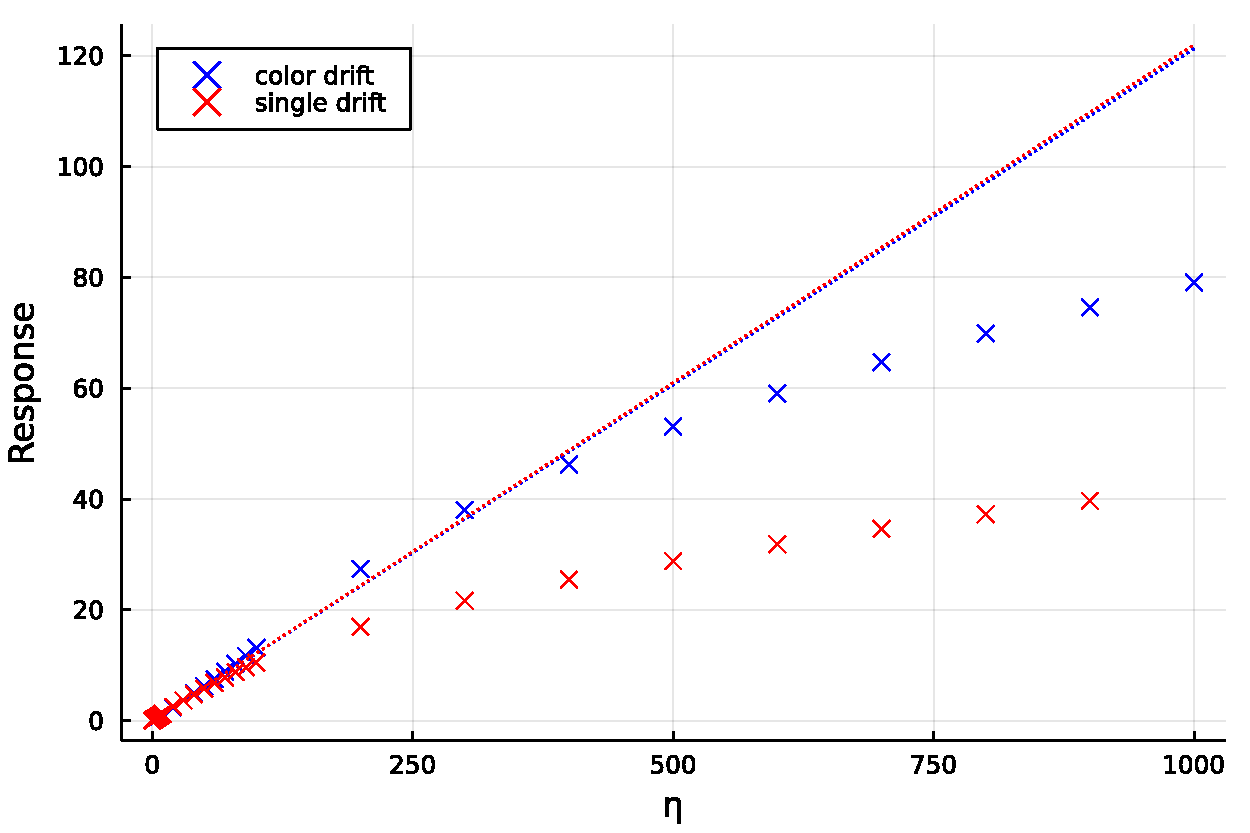
\includegraphics[width=0.7\linewidth]{figures/nemd/nemd_mobility_full.pdf}
      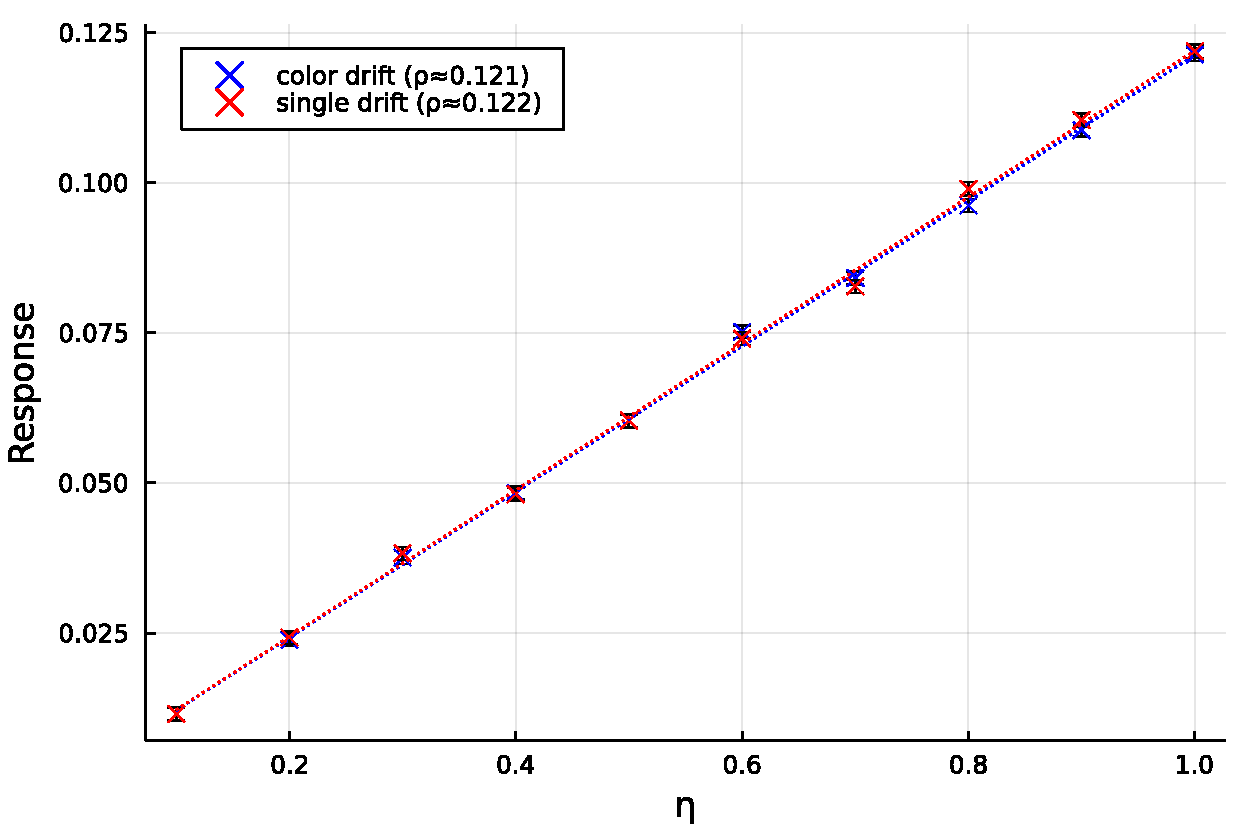
\includegraphics[width=0.7\linewidth]{figures/nemd/nemd_mobility_linear.pdf}
      \caption{ \label{fig:nemd_mobility_full}
        Average mobility response against forcing intensity for the Lennard-Jones system \eqref{eq:reference_thermo_condition}. Extrapolations of the linear response are plotted in dotted lines.
      }
    \end{center}
  \end{figure}

Estimating the transport coefficients using \eqref{eq:nemd_response_estimator} and the variance through \eqref{eq:var_of_lsq_fit}, we obtain 
\begin{equation}
    \rho_{F_{\mathrm{S}}}=0.12204\pm0.0009,\qquad \rho_{F_{\mathrm{C}}}=0.12128\pm0.0009,
\end{equation}
where $\pm$ denotes one standard deviation.
\subsection{Shear viscosity}
As a second example, we discuss the transverse force field method to compute the shear viscosity. The idea was originally introduced in \cite{GMS73}, although we base our presentation on the more recent article \cite{JS12}.
We refer to this paper for thorough statements and proofs.
Let us assume for notational simplicity that $M=m\Id$.
We consider a case of the dynamics \eqref{eq:general_nemd_dynamics} with a forcing which acts on the longitudinal ($x$) momenta, and is dependent on the transverse ($y$) positions.
More precisely, we fix a reference periodic function $F_y:L\mathbb{T}\longrightarrow \R$,
and index the state as \[\left(q_{i\alpha}\right)_{\substack{\leq i\leq N\\1\leq \alpha\leq d}},\qquad \left(p_{i\alpha}\right)_{\substack{\leq i\leq N\\1\leq \alpha\leq d}}.\]
The non-equilibrium dynamics is defined by the following expression for $F$:
\begin{equation}
    \label{eq:shear_viscosity_forcing}
    \forall\, 1\leq i\leq N,\,\forall\, 2\leq \alpha\leq d,\qquad F(q)_{i1}=f_y(q_{i2}),\qquad F(q)_{i\alpha}=0.
\end{equation}
The idea is that by imposing a forcing \textit{profile} in the $x$-direction, we observe a velocity profile in response, which depends on the $y$-coordinate.
\begin{remark}[Anisotropic friction]
    In fact the precise model considered in \cite{JS12} also imposes a separate friction coefficient $\gamma_x$ for the longitudinal fluctuation-dissipation part of the dynamics.
    This can be interpreted as a simple case of a generalized Langevin dynamics where the friction coefficient $\gamma$ is an anisotropic diagonal matrix, which does not pose any difficulties from the theoretical point of view.
    We therefore restrict our attention to the case where $\gamma$ is scalar.
\end{remark}
In order to make precise the response of the system, we define
\begin{equation}
    \label{eq:velocity_profile}
    u_x(Y)\defeq \underset{\varepsilon \to 0}{\lim} \, \underset{\eta \to 0}{\lim} \frac{L_y\E_\eta \left[\sum_{i=1}^N p_{i1}\chi_\varepsilon(q_{i2}-Y)\right]}{\eta mN}
\end{equation}
to be the linear response profile in the longitudinal velocity, where $(\chi_\varepsilon)_{\varepsilon>0}$ is an approximation to the identity (that is a sequence of smooth compactly supported test functions which converge to the Dirac delta function in the sense of distributions).
In practice, $u_x$ can be estimated from numerical trajectories by decomposing the domain $\mathcal D$ in a finite number of transverse slices,
 and measuring the average longitudinal velocity in each of these slices.
 The shear viscosity $\sigma$ is then defined by the differential equation
\begin{equation}
    \label{eq:shear_viscosity_relation_diffeq}
    -\sigma u_x''(Y)+\gamma \rho u_x(Y)=\rho f_y(Y),
\end{equation}
where $\rho= N/L^3$ is the particle density.
In fact, the solutions to \eqref{eq:shear_viscosity_relation_diffeq} are periodic, thus the magnitude of the linear response can be estimated from its Fourier coefficients.
Indeed, writing
\begin{equation}
    \label{eq:fourier_coefficient}
    c_k(h)=\frac{1}{L}\int_0^L h(s)\exp\left(\frac{2ik\pi s}{L}\right)\,\dif s
\end{equation}
for the $k$-th Fourier coefficient of a $L$-periodic function $h$, applying $c_k$ to \eqref{eq:shear_viscosity_relation_diffeq} gives
\begin{equation}
    \label{eq:fourier_relation_sv}
    \begin{aligned}
        &-\sigma c_k(u_x'')+\gamma\rho c_k(u_x)=\rho c_k(f_y),\\
        &(\sigma \left(2k\pi/L\right)^2 +\gamma \rho)c_k(u_x)=\rho c_k(f_y),\\
        &\sigma =\rho\left(\frac{c_k(f_y)}{c_k(u_x)}-\gamma\right)\left(\frac{L}{2k\pi}\right)^2
    \end{aligned}
\end{equation}
using $c_k(h'')=-\left(2k\pi/L\right)^2 c_k(h)$ in the second line.
The Fourier coefficient $c_k(u_x)$ can then be estimated directly from trajectory averages. this has the advantage of giving an estimation of the linear response in the general framework defined above, and avoiding the discretization error arising from the finite number of transverse slices.
To this effect, we define the response observables as empirical Fourier coefficients:
\begin{equation}
    \label{eq:nemd_shear_viscosity_response}
    R_k(q,p)=\frac{1}N\sum_{i=1}^N\frac{p_{i1}}{m}\exp\left(\frac{2ik\pi q_{i2}}{L}\right),
\end{equation}
and the corresponding transport coefficients
\begin{equation}
    \label{eq:shear_viscosity_tranpsort_coefficient}
    \rho_{F,k}=\underset{\eta\to 0}{\lim}\frac{\E_\eta[R_k(q,p)]}{\eta}.
\end{equation}
It is easy to show that for the sinusoidal forcing, the response velocity profile, solution to \eqref{eq:shear_viscosity_relation_diffeq}, is still sinusoidal, so that the Fourier response is a meaningful measure of the magnitude of the response in the velocity profile.
In practice, it is sufficient to consider $k=1$.
\begin{remark}
    To obtain better statistics, one may for the purpose of numerical simulations want to consider a periodic domain whose unit cell is still a cuboid, but with a side length in the longitudinal direction that is longer than in the transverse direction.
    In this case we simply replace $L$ by $L_y$ in the response observables, where $L_y$ is the length of the unit cell in the transverse direction.
\end{remark}
The shear viscosity can then be computed from equation \eqref{eq:fourier_relation_sv}, through
\begin{equation}
    \label{eq:shear_viscosity_nemd_estimator}
    \sigma=\rho\left(\frac{c_k(f_y)}{\rho_{F,k}}-\gamma\right)\left(\frac{L}{2k\pi}\right)^2,
\end{equation}
again only considering $k=1$ in practice. Numerically, $\rho_{F,k}$ can be approximated by an estimator of the form \eqref{eq:rho_F_nemd_estimator}.
In our numerical experiments, we consider the same three forcing profiles as in \cite{JS12}, namely:
\begin{enumerate}[(i)]
    \item A sinusoidal forcing profile \[f_y(u)=\sin\left(\frac{2\pi u}{L}\right),\]
    \item a piecewise constant forcing profile \[f_y(u)=\1_{u<\frac{L}2}-\1_{u\geq \frac{L}2},\]
    \item and a piecewise linear forcing profile \[f_y(u)=\frac{4}{L}\left(u-\frac{L}4\right)\1_{u<\frac{L}2}-\frac{4}L\left(\frac{3L}4-u\right)\1_{u\geq \frac{L}2}.\]
\end{enumerate}
These forcings have the advantage that the Fourier coefficients can be analytically computed. We record in Figure \ref{tab:fourier_coefficients} the value of the first Fourier coefficient $F_1$ for each of these forcings.
As in the case of mobility, we fix a reference thermodynamic condition,
\begin{equation}
    \label{eq:reference_thermo_condition_sv}
    T=0.8,\quad \rho=0.7,\quad \gamma=1.0,\quad N=1000.
\end{equation}

\begin{figure}
    \begin{center}
        \begin{tabular}{ |c|c|c|c| }\hline
            $f_y$ & Sinusoidal & Piecewise constant & Piecewise linear \\
            \hline
            $c_1(f_y)$ & $i/2$ & $2i/\pi$ & $-4/\pi^2$ \\
            \hline 
        \end{tabular}
        \caption{ \label{tab:fourier_coefficients}
            First Fourier coefficients for transverse forcing profiles.
          }
    \end{center}
\end{figure}

\section{The Green--Kubo method}
An alternative route to the perturbation method described above leverages a famous expression for the transport coefficient in terms of an integrated correlation function, or, in less technical language, in terms of the fluctuations at equilibrium of the response observable.
This is the Green--Kubo method, which we describe in this section. We consider the invariant measure for the non-equilibrium dynamics \eqref{eq:general_nemd_dynamics}. By Theorem \ref{thm:nemd_exst_invariant_measure}, there exists a unique invariant measure with density $\psi_\eta$.
For notational consistency, let us write $\psi_0$ for the density of the equilibrium measure~$\mu$. Then the following result holds. 
\begin{theorem}[Series expansion for the non-equilibrium steady state]
    \label{thm:nemd_steady_state_series}
    There exists $r>0$ such that for all $0<\eta<r$,
    \begin{equation}
    \label{eq:nemd_steady_state_series}
        \frac{\psi_\eta}{\psi_0}=\left(1+\eta(\widetilde{\cL} \Pi \cL_\gamma^{-1}\Pi)^*\right)^{-1}\1_{\mathcal E}=\left(1+\sum_{k=1}^{\infty}(-\eta)^k\left[(\tilde \cL \Pi\cL_\gamma^{-1}\Pi)^*\right]^k\right)\1_{\mathcal E},
    \end{equation}
    where $\widetilde{\cL}$ is defined by \eqref{eq:nemd_generator}, $\Pi$ is the equilibrium centering projector defined in \eqref{eq:equilibrium_projector}, and adjoints are taken in $L^2(\mu)$.
\end{theorem}
\begin{proof}[Sketch of proof]
    The second equality identifies the Neumann series on the right as the resolvent of $1+(\widetilde{\cL} \Pi \cL_\gamma^{-1}\Pi)^*$, provided $\eta$ is taken small enough.
    In fact, from the spectral theory of bounded operators, $r$ can be determined as the spectral radius of $(\widetilde{\cL} \Pi \cL_\gamma^{-1}\Pi)^*$ in the space of bounded operators $\mathcal{B}(L^2_0(\mu))$.
    The core of the argument lies in making the ansatz
    \begin{equation}
        \label{eq:nemd_measure_ansatz}
        \psi_\eta=\psi_0(1+\eta f_1+\eta^2 f_2+\dotsm).
    \end{equation}
    The stationary Fokker-Planck equation \eqref{eq:nemd_fp_equation} writes
    \[(\cL_\gamma +\eta \widetilde{\cL})^{\dagger}\psi_0(1+\eta f_1+\eta^2 f_2+\dotsm)=(\cL_\gamma +\eta \widetilde{\cL})^{*}(1+\eta f_1+\eta^2 f_2+\dotsm)=0.\]
    Indeed, for an arbitrary test function $\varphi$,
    \begin{align*}
        \int \left(\cL_\gamma +\eta \widetilde{\cL}\right)\varphi \psi_\eta &=0\\
        &=\int \left[\left(\cL_\gamma +\eta \widetilde{\cL}\right)\varphi\right](1+\eta f_1+\eta^2 f_2+\dots)\,\dif \mu\\
        &=\int \varphi \left[\left(\cL_\gamma +\eta \widetilde{\cL}\right)^*(1+\eta f_1+\eta^2 f_2+\dots)\right]\,\dif \mu.
    \end{align*}
    By formally identifying terms of the same degree in $\eta$, we obtain
    \begin{align*}
        \cL_\gamma^* \1_\mathcal E&=0,\\
        \widetilde{\cL}^*\1_{\mathcal E}+\cL_\gamma^*f_1&=0,\\
        \widetilde{\cL}^*f_1+\cL_\gamma^*f_2&=0,
    \end{align*}
    and so on. Note that the first equality is the equilibrium Fokker-Planck equation.
    Thus, by induction, again formally, we obtain.
    \begin{align*}
        f_1 &= (-\cL_\gamma^*)^{-1}\widetilde{\cL}^*\1_{\mathcal E},\\
        f_2 &= (-\cL_\gamma^*)^{-1}\widetilde{\cL}^*f_1,\\
        &\dotsm\\
        f_n &= \left[(-\cL_\gamma^*)^{-1}\widetilde{\cL}^*\right]^{n}\1_{\mathcal E},
    \end{align*}
    whence the formal proof follows, by observing that we can write 
    \[(-\cL_\gamma^*)^{-1}\widetilde{\cL}^*=-(\widetilde{\cL} \Pi \cL_\gamma^{-1}\Pi)^*.\]
    For a rigorous proof, several points should be made precise:
    \begin{enumerate}[(i)]
        \item The convergence of the series \eqref{eq:nemd_steady_state_series} for sufficiently small $\eta$, which can be obtained by showing the boundedness of the operator $(\widetilde{\cL} \Pi \cL_\gamma^{-1}\Pi)^*$ on $L_0(\mu)$.
        \item The fact that $\psi_0\left(1+\eta(\widetilde{\cL} \Pi \cL_\gamma^{-1}\Pi)^*\right)^{-1}\1_{\mathcal E}$ is indeed a solution to the stationary Fokker-Planck equation, and that it is indeed a probability density. This is done by showing that it is a positive function.
    \end{enumerate}
    One can then conclude by uniqueness of the steady-state probability measure.
\end{proof}
The linear response can be read off directly from the first term of the series expansion.
\begin{corollary}[Green--Kubo formula]
    Let $R$ be any response observable such that $\E_\mu[R]=0$, and $R\in L^{\infty}_{\mathcal{K}_n}$ for some $n$.
    Then we have the following formula for the linear response
    \begin{equation}
        \label{eq:green_kubo}
        \underset{\eta\to 0}{\lim}\,\frac{\E_{\eta}[R]}{\eta}=\int_0^\infty \E_\mu[R(q_t,p_t)S(q_0,p_0)]\dif t,
    \end{equation}
    where the expectation on the right hand side is with respect to all equilibrium dynamics trajectories with canonical initial distribution, and $S$ is defined by
    \begin{equation}
        \label{eq:conjugate_response}
        S=\widetilde{\cL}^*\1_{\mathcal E}=\beta F(q)\cdot M^{-1}p,
    \end{equation}
    and is called the conjugate response function. 
\end{corollary}
The latter expression follows from a simple integration by parts.
\begin{proof}
    By Theorem \ref{thm:nemd_steady_state_series}, we can write 
    \begin{align*}
        \underset{\eta\to 0}{\lim}\,\frac{\E_{\eta}[R]}{\eta}&=\int_{\mathcal E}R(q,p)\left((-\cL_\gamma^*)^{-1}\widetilde{\cL}^*\1_{\mathcal E}\right)(q,p)\psi_0(q,p)\,\dif q\, \dif p\\
        &=\int_{\mathcal E}\left[(-\cL_\gamma)^{-1}R\right](q,p)S(q,p)\psi_0(q,p)\,\dif q\, \dif p\\
        &=\int_{\mathcal E}\int_0^\infty\E^{(q,p)}[R(q_t,p_t)S(q_0,p_0)]\psi_0(q,p)\,\dif t\,\dif q\,\dif p\\
        &=\int_0^\infty \E_\mu[R(q_t,p_t)S(q_0,p_0)]\,\dif t,
    \end{align*}
    where we rely on an expression like \eqref{eq:resolvent_langevin} for $(-\cL_\gamma)^{-1}.$
\end{proof}
The Green--Kubo formula has a great advantage, in that it allows us to estimate the transport coefficients for as many different perturbations and response observables as we want \emph{from a single equilibrium trajectory}.
Indeed, one only needs to compute the corresponding integrated correlation functions \eqref{eq:green_kubo}.
\subsection{Numerical implementation}
We now describe a method to compute correlation functions necessary to the Green--Kubo method from a single long numerical trajectory.
This method is described by Tuckerman in~\cite[Section 13.4.2]{T10} for Hamiltonian trajectories.
In fact we consider a slight extension in which we let $R$ and $S$ to be vector-valued observables.
For notational simplicity, we assume that $R$ and $S$ are component-wise centered. The quantities we want to estimate are 
\begin{equation}
    \label{eq:time_correlation}
    C(t)=\E_\mu[R(q_t,p_t)^\intercal S(q_0,p_0)].
\end{equation}
We let $(q^n,p^n)_{n\geq 0}$ be a numerical trajectory, which we see as the random iterates of the Markov chain associated with a numerical scheme, with a regular timestep $\Dt>0$.
We further assume that the trajectory is stationary for this Markov chain, which is a realistic assumption if we equilibriate the system using our numerical scheme before recording states.
By stationarity, the equality in law
\[(q^n,p^n,q^0,p^0) \overset{\mathrm{law}}{=}(q^{n+k},p^{n+k}q^k,p^k)\]
for all $k\geq 0$. Hence we define the following estimator for $C(n\Dt)$, for $0\leq n\leq N_{\mathrm{iter}}:$
\begin{equation}
    \label{eq:ac_estimator}
    \widehat{C}_{N_{\mathrm{iter}}}(n\Dt) = \frac{1}{N_{\mathrm{iter}}-n+1}\sum_{k=0}^{N_{\mathrm{iter}}-n}R(q^{n+k},p^{n+k})^\intercal S(q^k,p^k).
\end{equation}
Note the quality of the estimators degrades with $n$. Thus in practice, we fix $N_{\mathrm{corr}}\ll N_{\mathrm{iter}}$, and compute these estimators for $0\leq n \leq N_{\mathrm{corr}}$.
Our implementation can be found in the Molly \cite{Molly} source code as the \verb|TimeCorrelationLogger| object and associated methods.
Using these estimators, we can estimate the transport coefficient through the Green--Kubo formula \eqref{eq:green_kubo}. The simplest way is to use a naive Riemann sum, or rectangle rule:
\[\rho_F \approx \Dt\sum_{k=0}^{N_{\mathrm{corr}}} \widehat{C}_{N_{\mathrm{iter}}}(k\Dt).\]
In fact, the analysis of \cite[Corollary 2.3]{LMS13} shows that using a trapezoidal rule reduces the error to $\mathrm{O}(\Dt^2)$ for integration schemes of weak order 2.
However, these procedures introduce a truncation in time of the integral in \eqref{eq:green_kubo}.
Another approach consists in extrapolating the behavior of $\widehat{C}_{N_{\mathrm{iter}}}$ by fitting a parametric model 
\begin{equation}
    \label{eq:time_correlation_parametric_model}
    C_{\theta}(t)=\left(\sum_{k=1}^{m}a_k\e^{-\lambda_k t}\cos(f_k t+\omega_k)\right),
\end{equation}
where \[\theta=(\lambda_k,a_k,f_k,\omega_k)\in \left(\R_+^*\times\R\times \R \times \R\right)^{m}\]
is the parameter. The form of this model is justified empirically, although a formal argument based on a diagonalisation of the evolution semigroup can be made, and using the conjugate symmetry property
$\cL_\gamma \overline{\psi}=\overline{\cL_\gamma \psi}$
for $\psi$ a complex-valued observable.
Rigorously justifying and quantifying the accuracy of this model requires fine knowledge of the spectrum of $\cL_\gamma$.
At any rate, we can then fit the model in a least-squares sense,
\begin{equation}
    \theta^*=\underset{\theta\in \left(\R_{+}^*\times\R\times \R \times \R\right)^{m}}{\mathrm{argmin}}\sum_{n=0}^{N_{\mathrm{corr}}}\left| C_{\theta}(n\Dt)-\widehat{C}_{N_{\mathrm{iter}}}(n\Dt) \right|^2,
\end{equation}
using gradient descent, or the Gauss-Newton method, and deduce an estimator for the transport coefficient,
\begin{equation}
    \label{eq:rho_F_estimator_GK_fit}
    \widehat{\rho}^{\mathrm{GK}}_{F,N_{\mathrm{iter}}}=\int_0^\infty C_{\theta^*}(t)\,\dif t,
\end{equation}
Using the simple identity
\begin{equation}
    \label{eq:int_analytic_form}
    a\int_0^{\infty}\e^{-\lambda t}\cos(ft+\omega)\,\dif t=a\frac{\lambda\cos \omega - f\sin\omega}{\lambda^2+f^2},
\end{equation}
we get a closed form for the estimator,
\[\widehat{\rho}^{\mathrm{GK}}_{F,N_{\mathrm{iter}}}=\sum_{k=1}^m a_k\frac{\lambda_k\cos \omega_k - f_k\sin\omega_k}{\lambda_k^2+f_k^2}.\]
\subsection{Mobility}
The Green--Kubo formula asserts that
\begin{equation}
    \label{eq:green_kubo_mobility}
    \underset{\eta\to 0}{\lim} \frac{\E_\eta[F\cdot M^{-1}p]}{\eta}=\beta \int_{0}^\infty \E_\mu[\left(F\cdot M^{-1}p_t\right)\left(F\cdot M^{-1}p_0\right)]\,\dif t.
\end{equation}
Using this expression, in the case of a mass-homogeneous system where the potential $V$ is of pair interaction form \eqref{eq:lennard_jones}, we can relate the transport coefficients for different forcings.
As a useful example, we compute an equation relating the transport coefficients for the single drift and color drift forcings. The argument is taken from unpublished notes by Julien Roussel.
\begin{example}[Relating linear responses]\label{ex:relating_linear_responses}
We assume $M=m\Id$. Let us define, for $1\leq i,j\leq N$,
\[c_{ij}=\frac{\beta}{m^2} \int_{0}^\infty \E_\mu[p_{i1,t}p_{j1,0}]\,\dif t.\]
By the form of the potential (Newton's third law), for all $q$,
\[\sum_{i=1}^N \frac{\partial}{\partial q_{i1}}V(q)=0.\]
This implies upon summing over $i$ the longitudinal $p$-components of the SDE \eqref{eq:langevin} and integrating
\begin{align*}\sum_{i=1}^N p_{i1,t}&= \sum_{i=1}^N \left[p_{i1,0}+\int_0^t \left(-\frac{\partial}{\partial q_{i1}}V(q_s)-\frac{\gamma}{m} p_{i1,s}\dif s +\sqrt{\frac{2\gamma}\beta}\dif W_{i1,s}\right)\right]\\
    &=\sum_{i=1}^N \left[p_{i1,0}-\frac{\gamma}{m}\int_0^t  p_{i1,s}\dif s +\sqrt{\frac{2\gamma}\beta} W_{i1,t}\right].\end{align*}
Multiply by $p_{11,0}$ and take the expectation with respect with the canonical initial distribution, the Brownian terms vanish, and we get
\begin{equation}
    \E_\mu\left[\left(\sum_{i=1}^N p_{i1,t}\right)p_{11,0}\right]=\sum_{i=1}^N\left[ \E_\mu\left[p_{i1,0}p_{11,0}\right]-\frac{\gamma}{m}\int_0^t \E_\mu\left[p_{i1,s}p_{11,0}\right]\dif s\right].
\end{equation}
By the decay properties of the evolution semigroup, the left hand side converges to $0$ as $t\to \infty$, while the integral is well-defined. Since $p_0$ has diagonal covariance with respect to $\mu$, we get
\begin{equation}
    \sum_{i=1}^N \frac{\gamma}m\int_0^\infty \E_\mu\left[p_{i1,s}p_{11,0}\right]\dif s=\E_\mu[p_{11,0}^2]=\frac{m}{\beta}.
\end{equation}
Equivalently, 
\[\sum_{i=1}^N c_{i1}=\frac{1}{\gamma}.\]
Using the indistinguishability property
 \[c_{ii}=c_{11},\qquad c_{ij}=c_{12}\] for all $i\neq j$,
 we can rewrite this identity as 
 \begin{equation}\label{eq:c12_c11_relation}c_{12}=\frac{1}{N-1}\left(\frac{1}{\gamma}-c_{11}\right).\end{equation}
Using this computation, we can relate the linear responses of the single drift and the color drift.
By the Green--Kubo formula, the transport coefficient for the single drift is given by $c_{11}$,
\[\rho_{F_{\mathrm{S}}}=c_{11}.\]
For the color drift, we expand, by the Green--Kubo formula,
\[\rho_{F_{\mathrm{C}}}=\frac{\beta}{m^2} \int_0^\infty \E_\mu[\left(F_{\mathrm{C}}\cdot p_t\right)\left(F_{\mathrm{C}}\cdot p_0\right)]\,\dif t=\frac1N\left(\sum_{i=1}^N c_{ii} + 2\sum_{1\leq i< j\leq N}(-1)^{i+j}c_{ij}\right)\]
By indistinguishability, and using
\[2\sum_{1\leq i\neq j\leq N}(-1)^{i+j}=-2\left\lfloor \frac{N}{2}\right\rfloor,\]
which is easily seen by induction, we get
\begin{equation}
    \rho_{F_{\mathrm{C}}}=c_{11}-\frac{2\lfloor N/2 \rfloor}{N(N-1)}\left(\frac1{\gamma}-c_{11}\right).
\end{equation}
\end{example}
Note that this analysis is consistent with what we observe numerically, although because of persisting statistical uncertainty, much longer trajectories (or smaller systems) have to be considered to confirm this relation numerically.
Let us also mention that the discrepancy vanishes in the thermodynamic limit, at rate $\mathrm{O}(N^{-1})$.
Since the system we consider is isotropic, we also have 
\[c_{11}=\frac{\beta}{m^2}\int_0^\infty\E_\mu[p_{i\alpha,s}p_{i\alpha,0}]\,\dif s\]
for any $1\leq i\leq N$ and $1\leq \alpha\leq d$. Thus, the mobility can be computed through an expression of the form \eqref{eq:time_correlation}:
\begin{equation}
    \label{eq:diffusion_gk_scalar_product}
    \rho_{F_{\mathrm{S}}}=c_{11}=\frac{\beta}{m^2 d N}\int_{0}^\infty \E_\mu[p_s^\intercal p_0]\,\dif s,
\end{equation}
which is the Green--Kubo relation we use in our numerical experiments.
We expect that the expression \label{eq:diffusion_gk_scalar_product} is much better in terms of asymptotic variance than the naive Green--Kubo estimator based on \eqref{eq:green_kubo_mobility}.
We confirm this fact empirically, in the sense that the estimator based on \eqref{eq:diffusion_gk_scalar_product} converges much quicker, although further work should be undertaken to study this effect systematically.
In Figure \ref{fig:gk_mobility}, we plot the velocity autocorrelation function used in the estimator \eqref{eq:diffusion_gk_scalar_product}, and its integral. 
We used the same thermodynamics conditions as for the NEMD method \eqref{eq:reference_thermo_condition}. 
In Figure \ref{fig:fit_gk_mobility}, we show the fitted non-linear least squares model \eqref{eq:time_correlation_parametric_model} for the autocorrelation function, using $m=4$ modes, trained using the Gauss--Newton algorithm.
The estimated correlation function was obtained from a single numerical trajectory with a physical reduced time of $t_{\mathrm{fin}}=1.628 \times 10^5$.
The corresponding estimated values for the mobility are $0.1218$ based on a trapezoid quadrature of the truncated autocorrelation function, and $0.1217$ for the analytic integral of the parametric model.


\begin{figure}[htbp]
    \begin{center}
      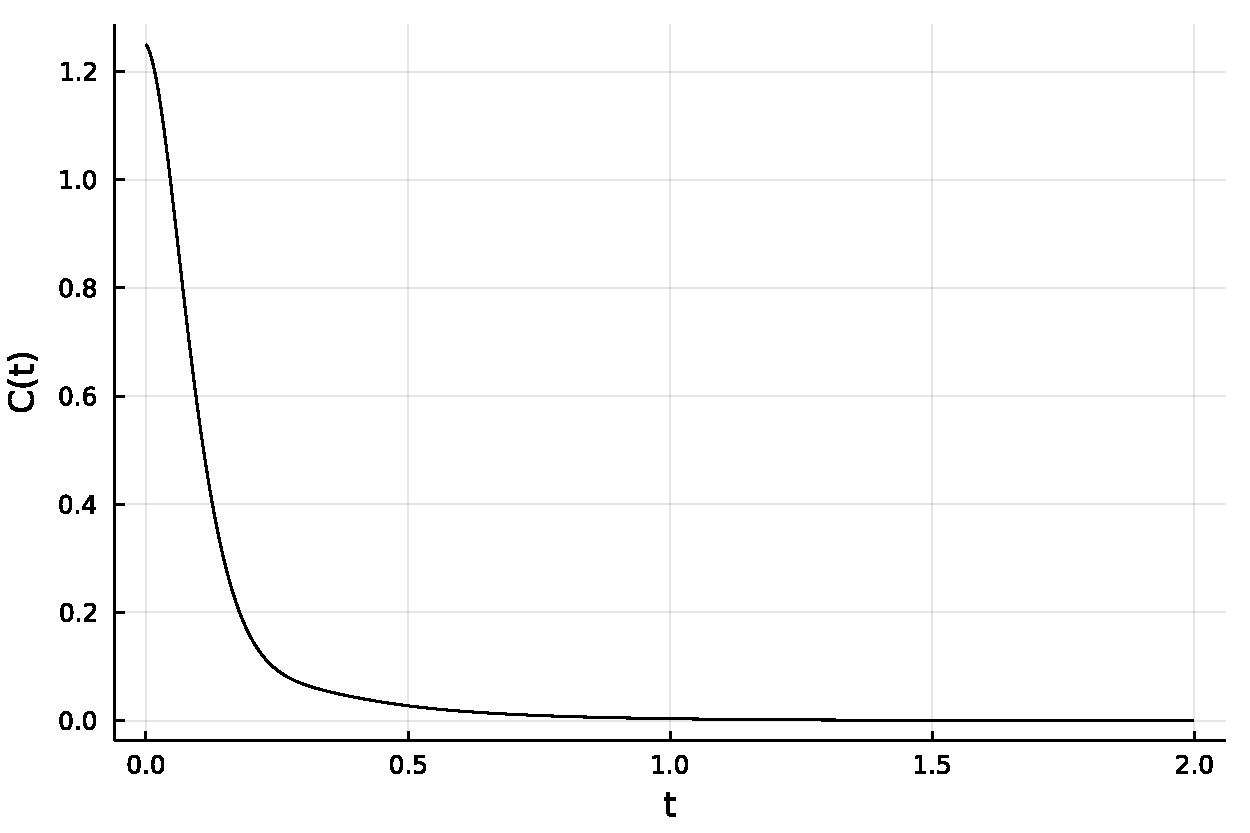
\includegraphics[width=0.7\linewidth]{figures/autocorr.pdf}
      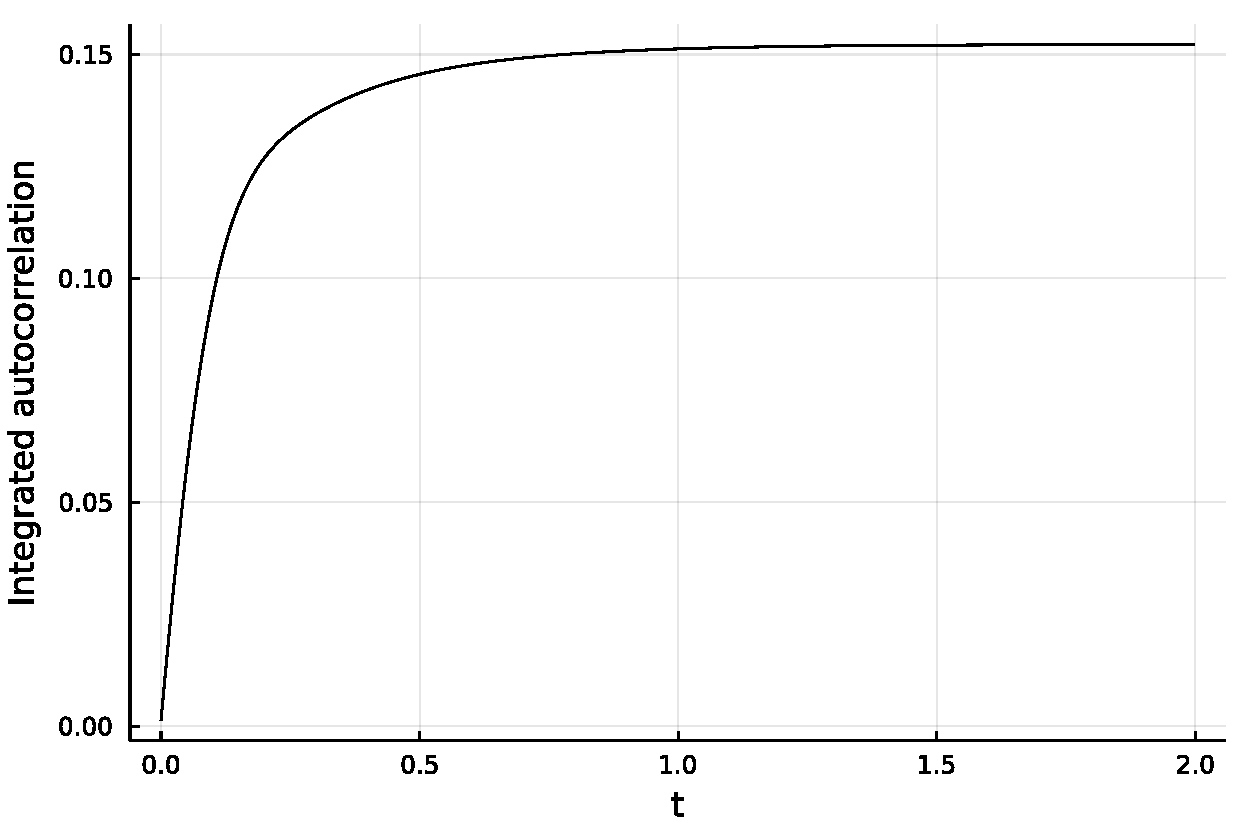
\includegraphics[width=0.7\linewidth]{figures/int_autocorr.pdf}
      \caption{ \label{fig:gk_mobility}
        Velocity autocorrelation function (top) and its integral (bottom) for the Lennard-Jones system \eqref{eq:reference_thermo_condition}.
      }
    \end{center}
  \end{figure}

  \begin{figure}[htbp]
    \begin{center}
      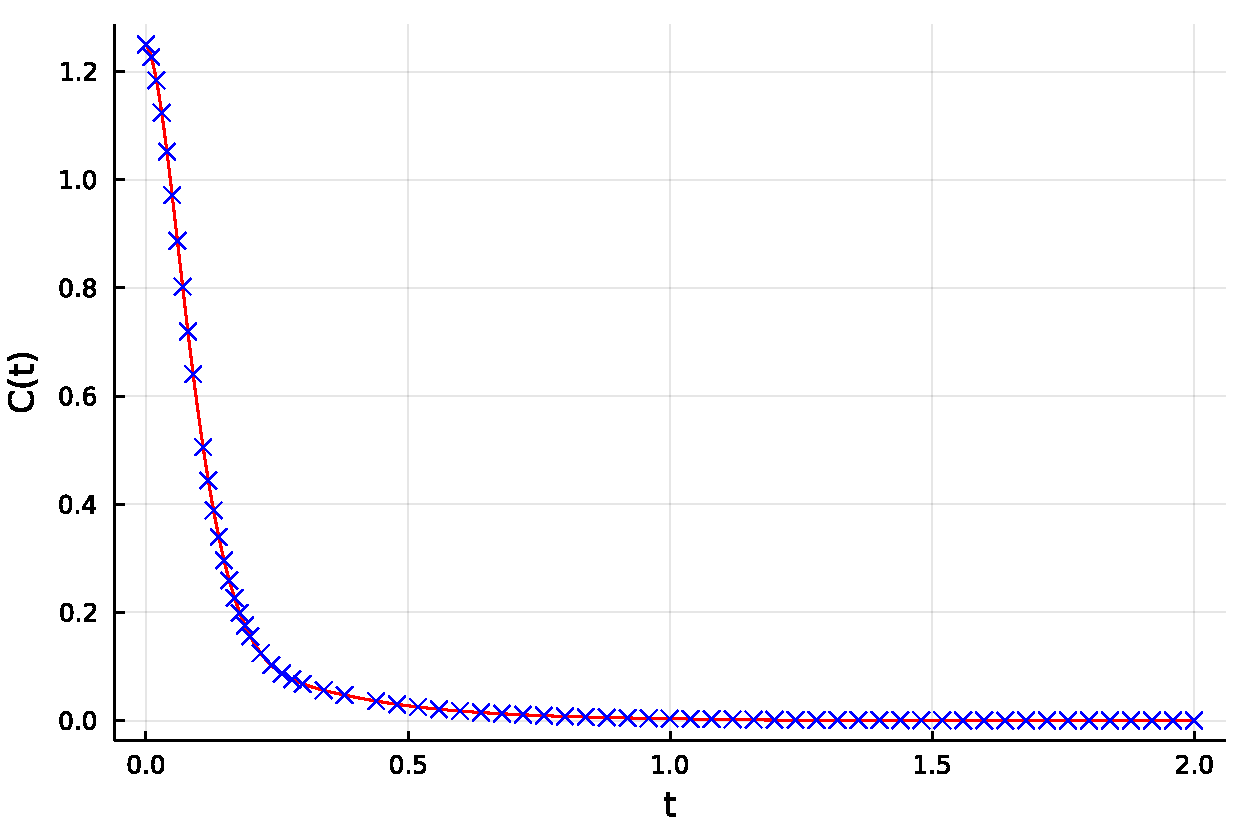
\includegraphics[width=0.8\linewidth]{figures/autocorr_fit.pdf}
      \caption{ \label{fig:fit_gk_mobility}
        Fitted parametric model \eqref{eq:time_correlation_parametric_model} (in dotted line) superimposed on autocorrelation function from Figure \ref{fig:gk_mobility} (in black) for the Lennard-Jones system \eqref{eq:reference_thermo_condition}.
      }
    \end{center}
  \end{figure}

We conclude this section on mobility computations by the discussion of a final method, which yields a nice physical interpretation for the mobility.
\begin{remark}[Einstein relation for mobility]
    Recalling the computations in Section \ref{subsec:asymptotic_variance_cont}, we can write, for $R$ a centered response observable,
    \begin{equation}
        \E_\mu\left[\left(\frac1{\sqrt{T}}\int_0^T R(q_t,p_t)\,\dif t\right)^2\right]=2\int_0^T \E_\mu\left[R(q_t,p_t)R(q_0,p_0)\right]\left(1-\frac{t}T\right)\,\dif t.
    \end{equation}
    Assuming an exponential decay of the evolution semigroup, we get 

    \begin{equation}
        \label{eq:einstein_formula}
        \int_0^\infty\E_\mu\left[R(q_t,p_t)R(q_0,p_0)\right]\,\dif t=\underset{T\to\infty}{\lim}\,\frac{1}{2T}\E_\mu\left[\left(\int_0^T R(q_t,p_t)\,\dif t\right)^2\right].
    \end{equation}
    This is the Einstein formula. In the case of mobility $R(q,p)=F\cdot M^{-1}p$, the right-hand side rewrites 
    \begin{equation}
        \label{eq:einstein_formula_mobility}
        \underset{T\to\infty}{\lim}\,\frac{1}{2T}\E_\mu\left[\left(F\cdot \left(Q_T-Q_0\right)\right)^2\right],
    \end{equation}
    where 
    \begin{equation}
        \label{eq:self_diffusion_process}
        Q_t=Q_0+\int_0^t M^{-1}p_s\,\dif s=\int_0^t \,\dif q_s
    \end{equation}
    is the so called \textbf{self-diffusion} process, which formally satisfies the same SDE as $q$, but in the unperiodic domain $\R^{dN}$. 
    Its trajectories corresponds to the unwrapped or unperiodized trajectories of the coordinates, which makes them particularly easy monitor during a numerical simulation.
    This terminology is justified by a result, \cite[Theorem 1]{R89}, asserting that the diffusively rescaled self-diffusion process 
    \[\sqrt{\varepsilon}(Q_{\varepsilon^{-1}t}-Q_0)\]
    converges in law as $\varepsilon \to 0$ to a Brownian motion with diffusion matrix $\mathfrak D$ characterized by
    \begin{equation}
        \label{eq:diffusion_tensor}
        F\cdot \mathfrak D F= \underset{T\to\infty}{\lim}\,\frac{1}{T}\E_\mu\left[\left(F\cdot \left(Q_T-Q_0\right)\right)^2\right].
    \end{equation}
    In the case of an isotropic system, the diffusion matrix is characterized by a single number, the diffusion coefficient, which is given by the half normalized trace of the diffusion matrix.
    \begin{equation}
        \label{eq:diffusion_coefficient}
        D=\frac{1}{2dN}\mathrm{Tr}(\mathfrak D)=\underset{T\to\infty}{\lim}\,\frac{1}{2dNT}\E_\mu\left[\left|Q_T-Q_0\right|^2\right]
    \end{equation}
    In view of the Einstein relation \eqref{eq:einstein_formula_mobility} and of the Green--Kubo relation \eqref{eq:green_kubo_mobility}, the mobility is related to the diffusion coefficient as
    \begin{equation}
        \label{eq:mobility_from_einstein}
        \rho_{F_{\mathrm{S}}}=\beta D.
    \end{equation}
\end{remark}
    The formula \eqref{eq:diffusion_coefficient} provides a new family of estimators for the mobility, based on a computation of the self-diffusion coordinates expression \eqref{eq:diffusion_coefficient}.
    In Figure \ref{fig:einstein_demo} we illustrate the strategy we used to compute the mobility using the Einstein formula, which we proceed to explain.
    We define the mean-squared deviation as the process
    \begin{equation}
        \label{eq:mean_squared_deviation}
        M_t=\frac{|Q_t-Q_0|^2}{dN}.
    \end{equation}
    Fixing a number of independent realizations $N_{\mathrm{run}}$ and a number of simulation iterations $N_{\mathrm{iter}}$, we consider, for each $i=1,\dots,N_{\mathrm{run}}$, a numerical trajectory of regularly sampled points from the mean-squared deviation,
    $M^i=(M^{i,k})_{0\leq k\leq N_{\mathrm{iter}}}.$ 
    These correspond to points sampled at regular time intervals $T_{\mathrm{samp}}=N_{\mathrm{samp}}\Dt$, where $\Dt$ is the simulation timestep, and computed from the numerical trajectory of the self-diffusion coordinates.
    We then obtain $N_{\mathrm{run}}$ estimators for $D$ by a linear regression on the mean-squared deviation trajectories, 
    \begin{equation}
        \widehat{D}^i_{N_{\mathrm{iter}}}= \frac{1}{2|\tau|^2} \tau\cdot M^i,
    \end{equation}
    where \[\tau=(kT_{\mathrm{samp}})_{0\leq k\leq N_{\mathrm{iter}}}\]
    is the vector of sampling times. An estimator for $D$, and thus for $\rho_{F_{\mathrm{S}}}$, is obtained by averaging over the number of independent runs:
    \begin{equation}
        \label{eq:diffusion_final_estimator}
        \widehat{D}_{N_{\mathrm{iter}}}=\frac{1}{N_{\mathrm{run}}}\sum_{i=1}^{N_{\mathrm{run}}}\widehat{D}^i_{N_{\mathrm{iter}}}.
    \end{equation}
    Nearly independent runs can be computed over a single trajectory, using for all $T,t\geq 0$ the stationarity
    \[(Q_T-Q_0)_{T\geq 0} \sim (Q_{T+t}-Q_t)_{T\geq 0},\]
    and the asymptotic independence, or decorrelation, between $(Q_{T+t}-Q_t)_{T\geq 0}$ and $(Q_s)_{0\leq s\leq t}$.
    This can be very simply exploited in a simulation, by resetting the self-diffusion coordinates to zero following each sample run. 
    In practice, one has to take care to take $N_{\mathrm{samp}}$ large enough so that the mean-squared deviation behaves approximately linearly over the sample time range $[0,T_{\mathrm{samp}}]$.
    In Figure \ref{fig:einstein_demo}, we illustrate the principle underlying this method. 
    For our final computation, we used $N_{\mathrm{run}}=545$, $N_{\mathrm{iter}}=10^6$, $\Dt=10^{-3}$, $N_{\mathrm{samp}}=1$.
    The estimated mobility is 
    \begin{equation}
        \label{eq:einstein_est_mobility}
        \rho_{F_{\mathrm{S}}}=0.12157\pm 0.00011,
    \end{equation}
    with error bars obtained using the empirical variance.
\begin{figure}[htbp]
    \begin{center}
      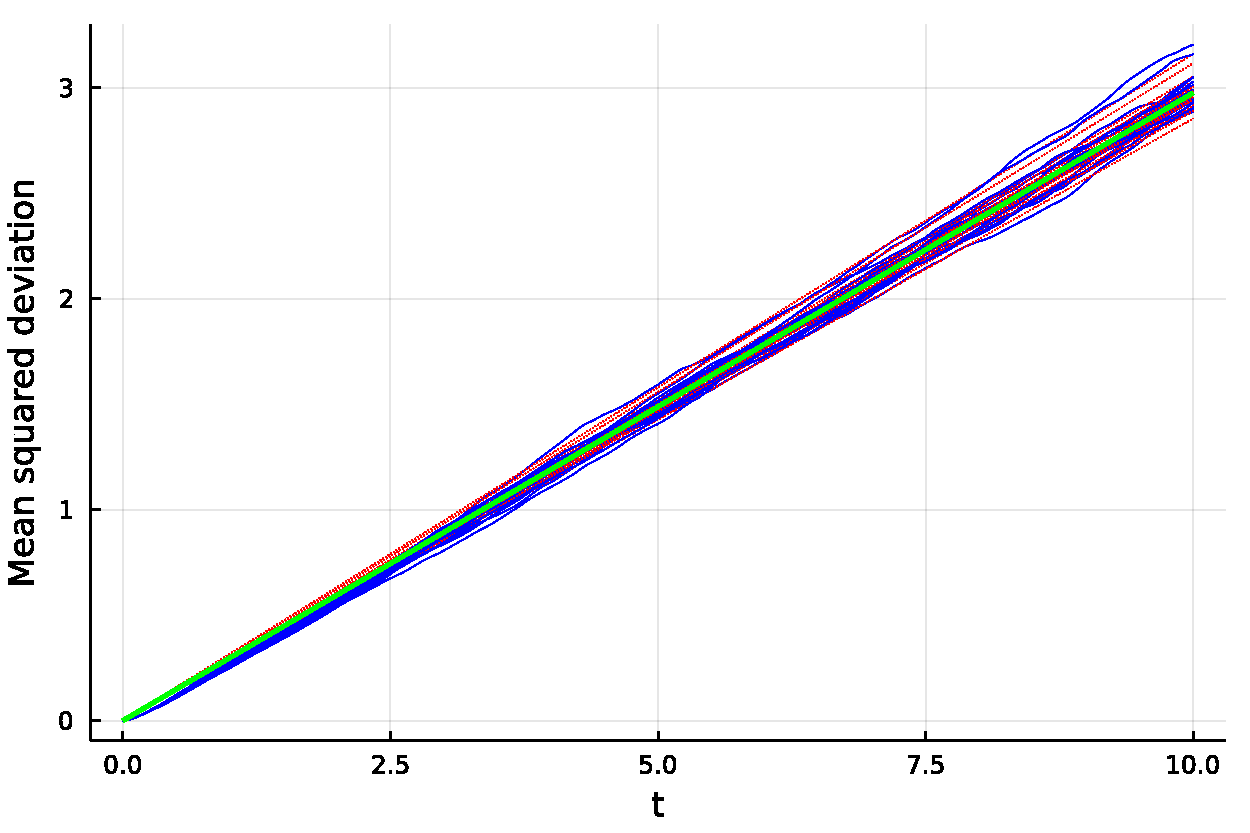
\includegraphics[width=0.8\linewidth]{figures/einstein_demo.pdf}
      \caption{ \label{fig:einstein_demo}
        Twenty independent realizations of the mean squared-deviation (in blue) superimposed with their corresponding linear regression lines (in red dotted lines).
        The regression line corresponding to the corresponding estimator \eqref{eq:diffusion_final_estimator} is plotted in bright green.
      }
    \end{center}
  \end{figure}
\subsection{Shear viscosity}
We conclude by applying the Green--Kubo formula to shear viscosity computations. It asserts, with $\rho_{F,k}$ given by \eqref{eq:shear_viscosity_tranpsort_coefficient},
\begin{equation}
    \label{eq:green_kubo_viscosity}
    \rho_{F,k}=\beta\int_0^\infty \E_\mu\left[R_k(q_t,p_t)\left(F(q_0)\cdot M^{-1}p_0\right)\right],
\end{equation}
where $R_k$ is given by \eqref{eq:nemd_shear_viscosity_response}.
At this point, let us remark that we can, similar to the mobility case in \eqref{eq:diffusion_gk_scalar_product}, exploit the isotropy of the equilibrium measure to our statistical advantage.
To do this let us define versions of the transverse forcing method for any pair of orthogonal canonical directions in $\R^d$. More precisely,
we define, for any $1\leq \alpha \neq \beta \leq d$,
\begin{align*}
    &R_{k,\alpha\beta}(q,p)=\frac{1}N\sum_{i=1}^N\frac{p_{i\alpha}}{m}\exp\left(\frac{2ik\pi q_{i\beta}}{L}\right),\\
    &F_{\alpha\beta}(q)_{i\alpha}=f_y(q_{i\beta}),\qquad F_{\alpha\beta}(q)_{i\delta}=0,\,\forall\, 1\leq i\leq N,\, \forall\, \delta \neq \beta.
\end{align*}

Then, by isotropy, we have
\begin{equation}
    \label{eq:green_kubo_viscosity_isotropic}
    \rho_{F,k}=\frac{\beta}{d(d-1)}\sum_{1\leq \alpha\neq\beta \leq d}\int_0^\infty\E_\mu\left[R_{k,\alpha\beta}(q_t,p_t)\left(F_{\alpha\beta}(q_0)\cdot M^{-1}p_0\right)\right].
\end{equation}

This can be rewritten as an expression of the form \eqref{eq:time_correlation}, with $d(d-1)$-dimensional observables. 
When $d=3$, the speedup in convergence is appreciable, though we made no attempt to quantitatively measure it.
We also take advantage of this opportunity to demonstrate the power of the Green--Kubo method by computing transport coefficients for all three forcing profiles using a single numerical trajectory.
In Figure \eqref{fig:sv_correlations}, we plot the correlation functions and corresponding integral for the three different forcing profiles.
We note that the results are roughly consistent with the analytic computations of Figure \ref{tab:fourier_coefficients}, in the sense that the normalized transport coefficient 
\[\frac{\rho_{F,k}}{c_k(f_y)}\]
should be real and positive. 
The persistance of an imaginary component in the estimation of this normalized transport coefficient can be attributed to statistical error, and is useful as a direct empirical non-convergence test for the Green--Kubo estimator.
Computations were run under the reference thermodynamic condition \eqref{eq:reference_thermo_condition_sv}, for a physical simulation time of $t_{\mathrm{fin}}=2.46\times 10^4$, with a timestep $\Dt=10^{-3}$ and a number of decorrelation steps $N_{\mathrm{corr}}=10^4$.
The corresponding estimates for the normalized transport coefficients are respectively $0.644$, $0.645$ and $0.655$ for the sinusoidal, piecewise constant and piecewise linear forcing profiles.

\begin{figure}[htbp]
    \begin{center}
      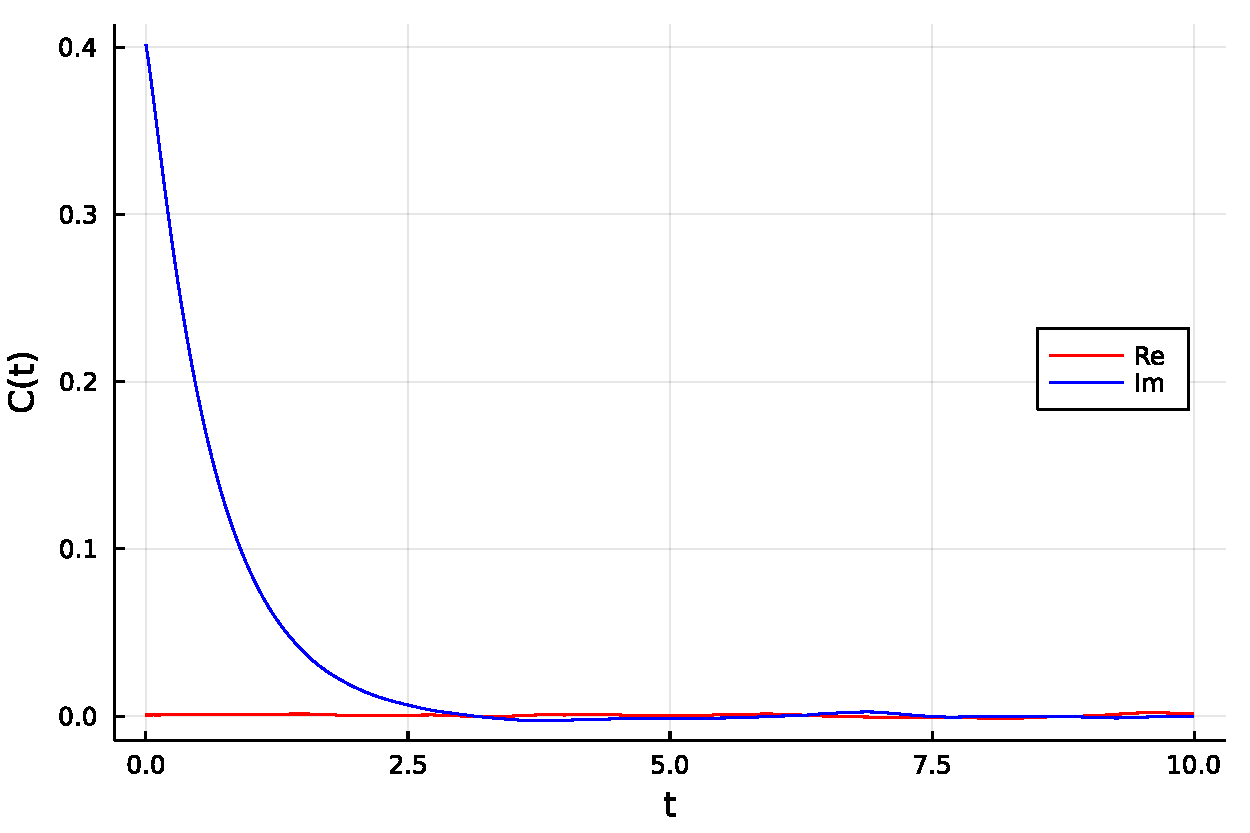
\includegraphics[width=0.49\linewidth]{figures/sinus_corr.pdf} 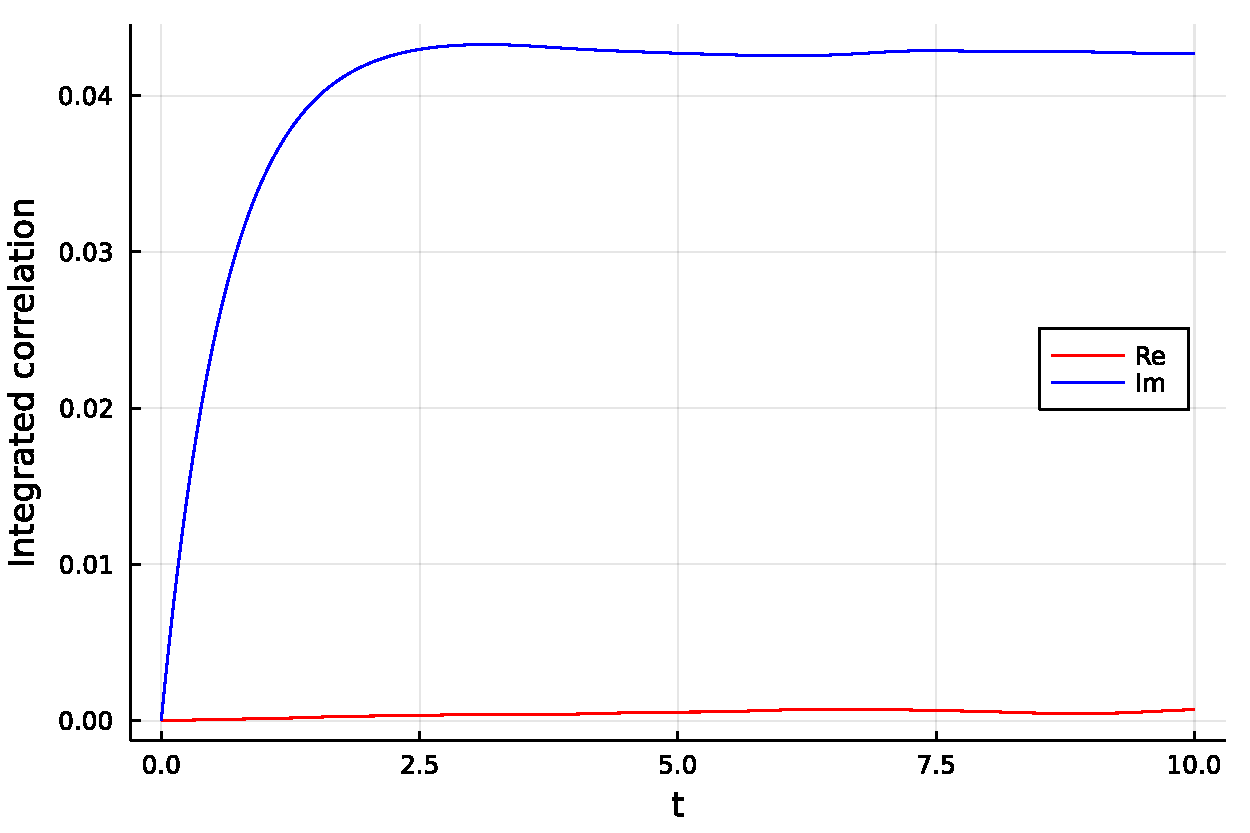
\includegraphics[width=0.49\linewidth]{figures/sinus_int_corr.pdf}
      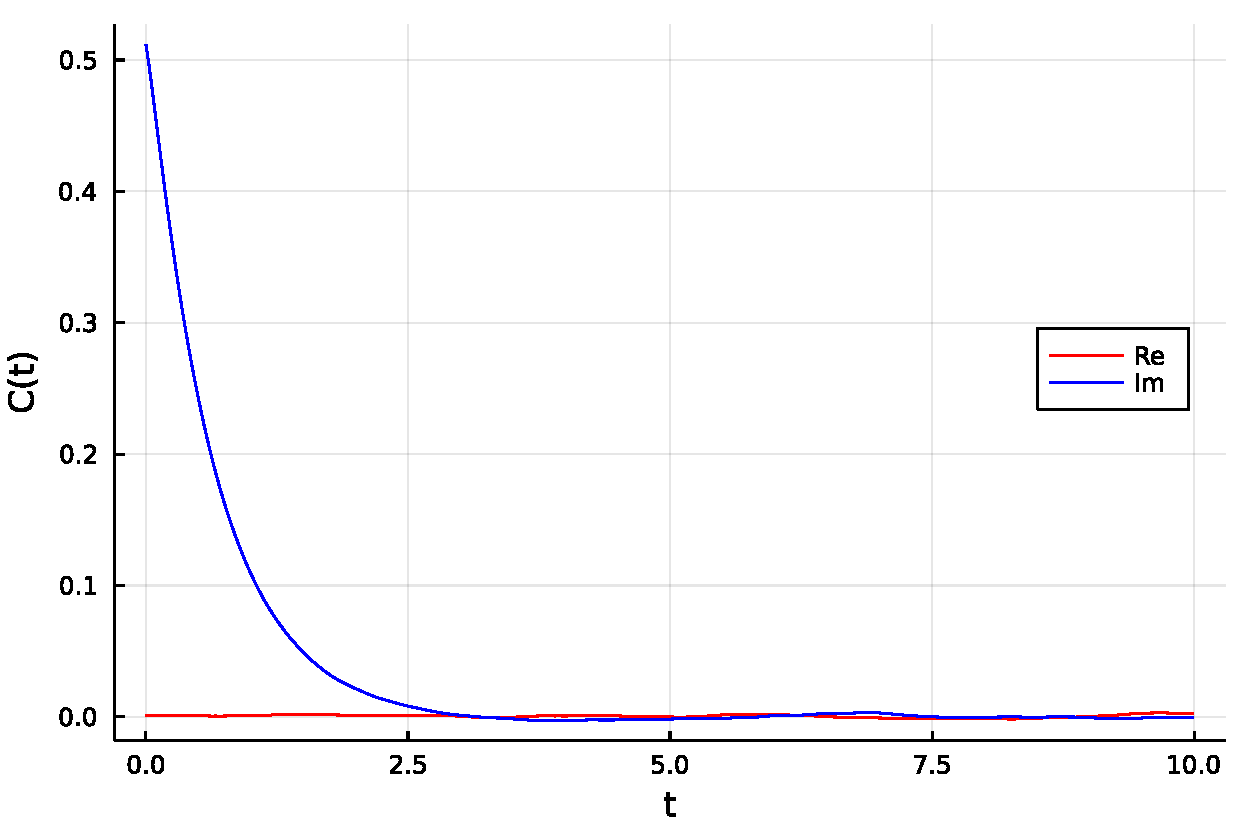
\includegraphics[width=0.49\linewidth]{figures/const_corr.pdf} 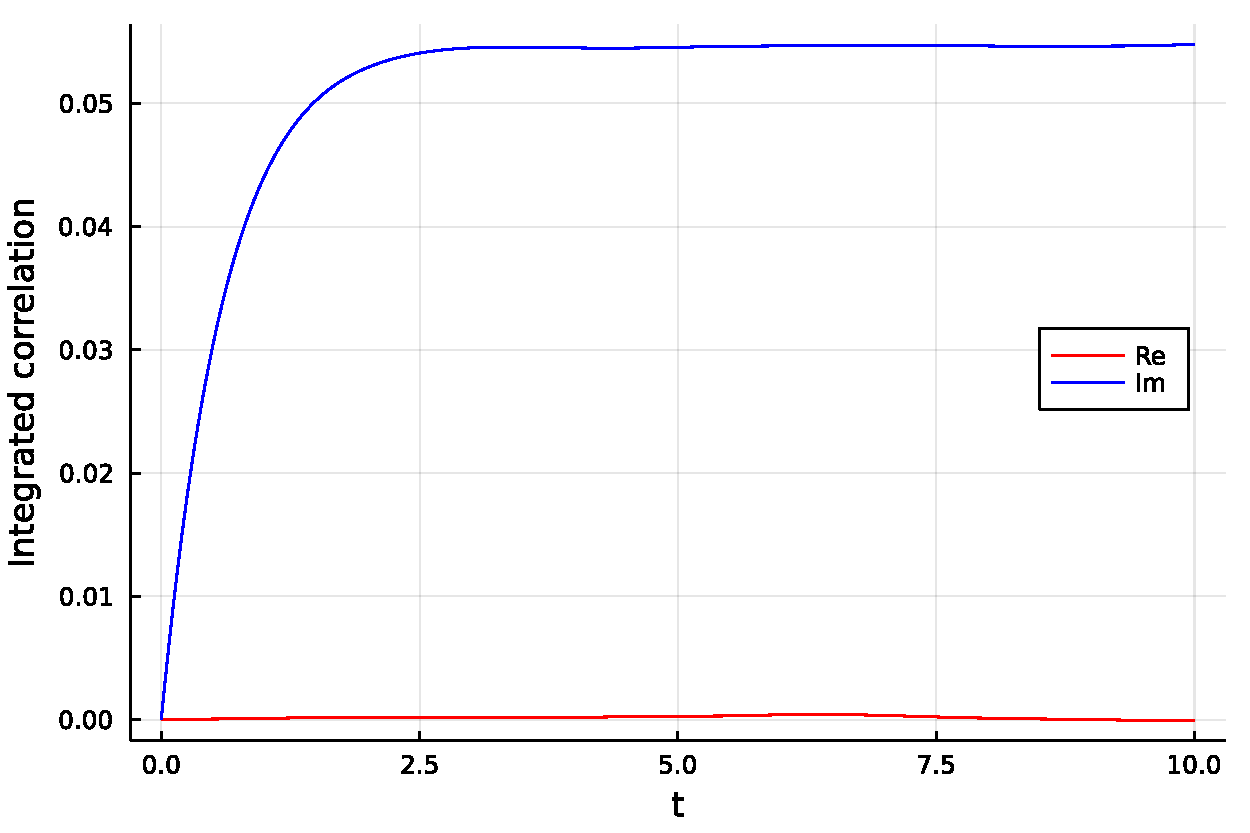
\includegraphics[width=0.49\linewidth]{figures/const_int_corr.pdf}
      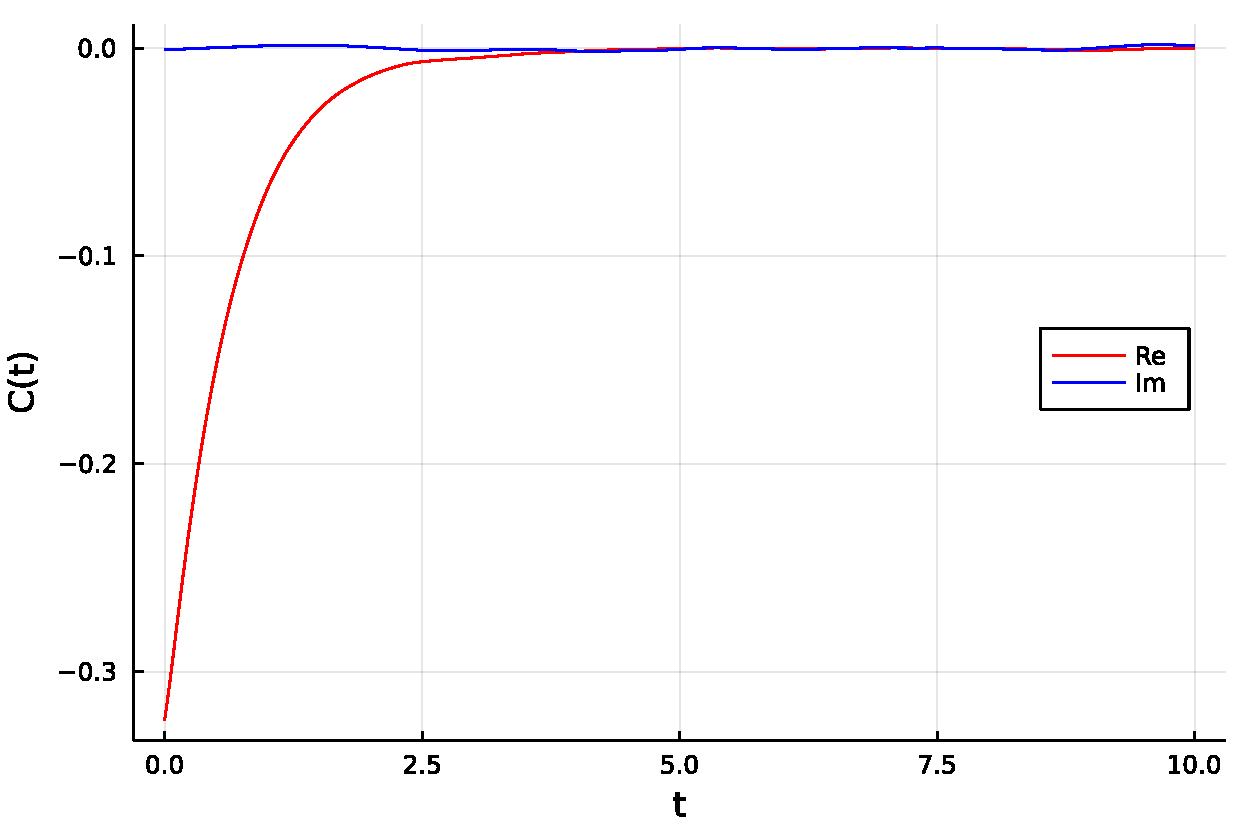
\includegraphics[width=0.49\linewidth]{figures/lin_corr.pdf} 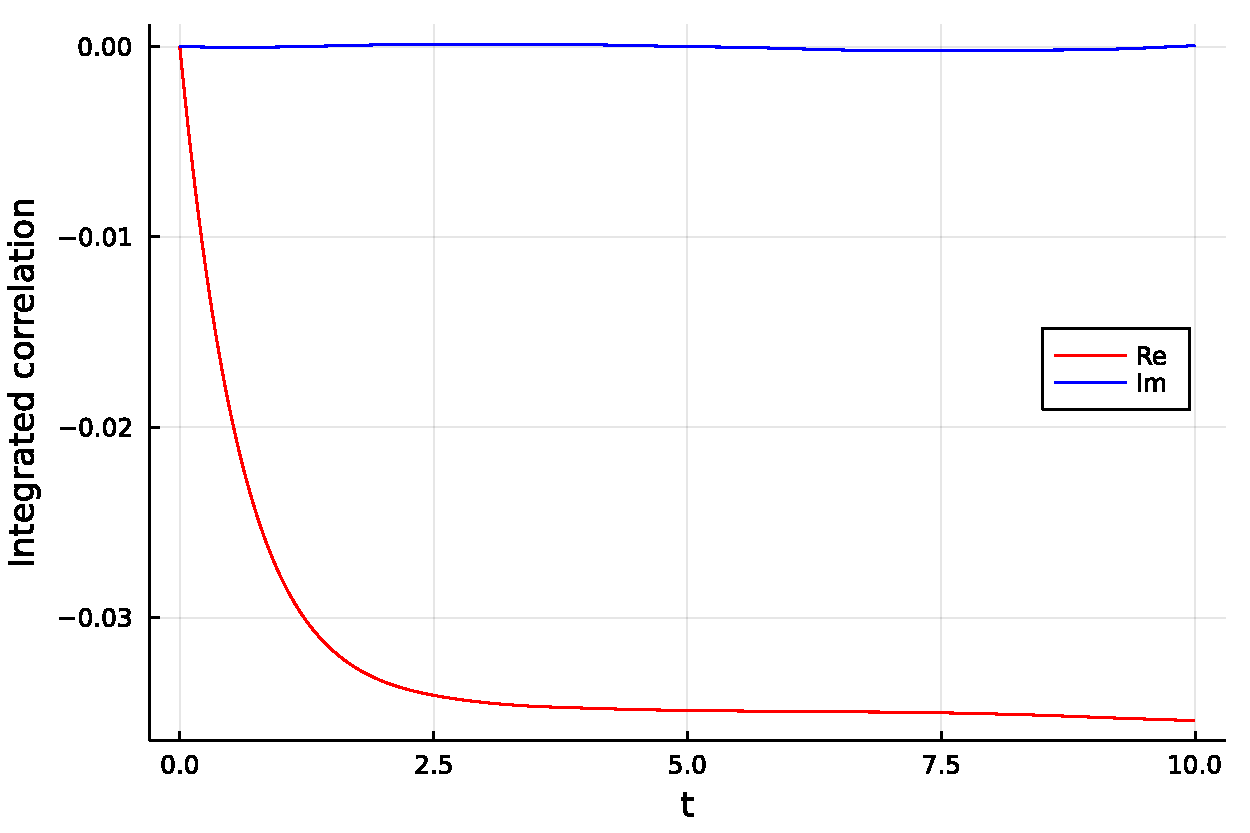
\includegraphics[width=0.49\linewidth]{figures/lin_int_corr.pdf}
      \caption{ \label{fig:sv_correlations}
        Correlation functions (left) and corresponding integrated correlation functions (right) for the shear viscosity dynamics. Top row: sinusoidal forcing, middle row: piecewise constant forcing, bottom row: piecewise linear forcing.
        Real parts are plotted in red and imaginary parts are plotted in blue. Integrals were obtained with a trapezoid rule.
      }
    \end{center}
  \end{figure}